\section{Gambaran Umum}
\label{sec:gambaran-umum}

Kabupaten Maluku Barat Daya adalah salah satu kabupaten dari Provinsi Maluku. Lokasinya yang jauh dari pusat provinsi (Kota Ambon) dan lebih dekat ke Timor Leste membuatnya tercakup dalam daerah 3T (Tertinggal, Terdepan dan Terluar). Jumlah penduduk Kabupaten MBD sekitar 91.387 jiwa dengan PDRB per kapita sebesar 23,96 Juta per tahun.

\begin{figure}[ht!]
    \centering
    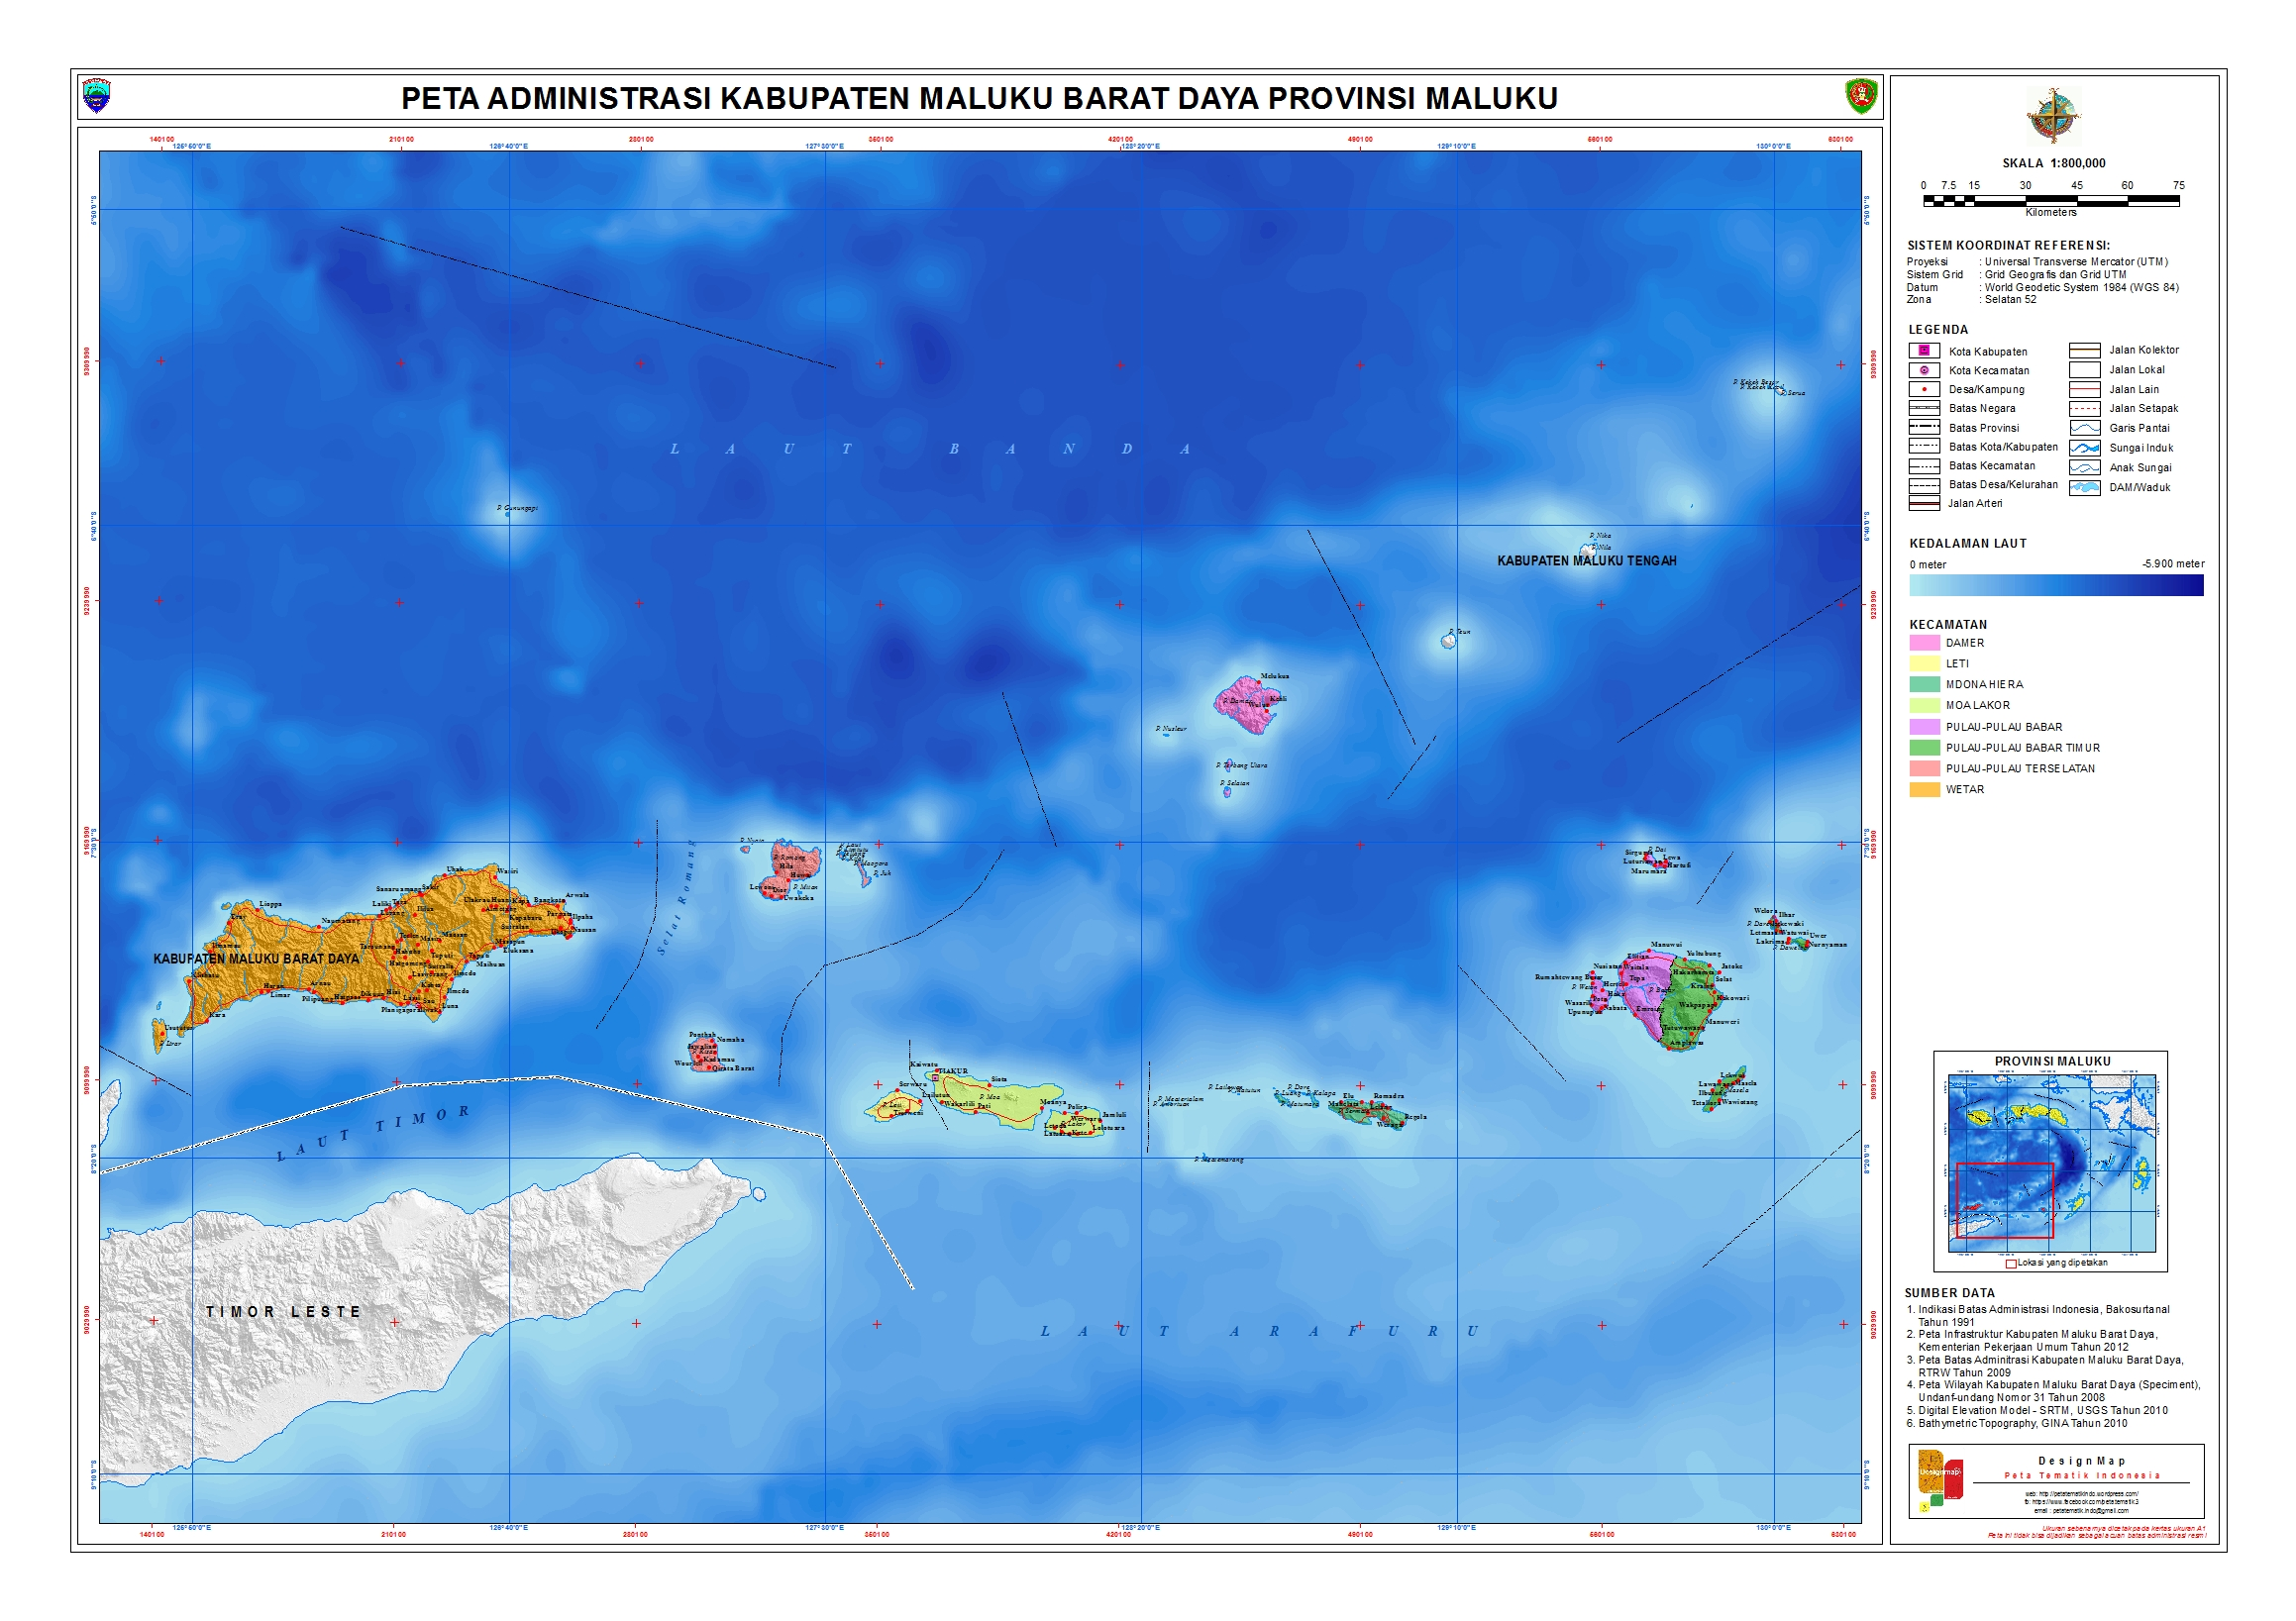
\includegraphics[width=0.8\textwidth]{gambar/administrasi-maluku-barat-daya-a1.jpg}
    \caption{Peta Administrasi Kabupaten Maluku Barat Daya \citep{Peta_Tematik_Indonesia_2014}}
    \label{fig:peta-mbd-basic}
\end{figure}

\subsection{Sistem Penyaluran BBM Kabupaten Maluku Barat Daya}
\label{subsec:sistem-eksisting}

    Kebutuhan BBM Kabupaten Maluku Barat Daya dilayani oleh Terminal Bahan Bakar Minyak Saumlaki didalam cakupan PT. Pertamina Patra Niaga Regional Maluku Papua. Berdasarkan SK Kepala BPH Migas No 55 Tahun 2019 dan realisasi pemasokan yang dilakukan oleh PT. Pertamina (Persero) didapatkan data pasokan BBM seperti gambar \ref{fig:realisasi-bbm-mbd}.

\begin{figure}[htbp!]
    \centering
    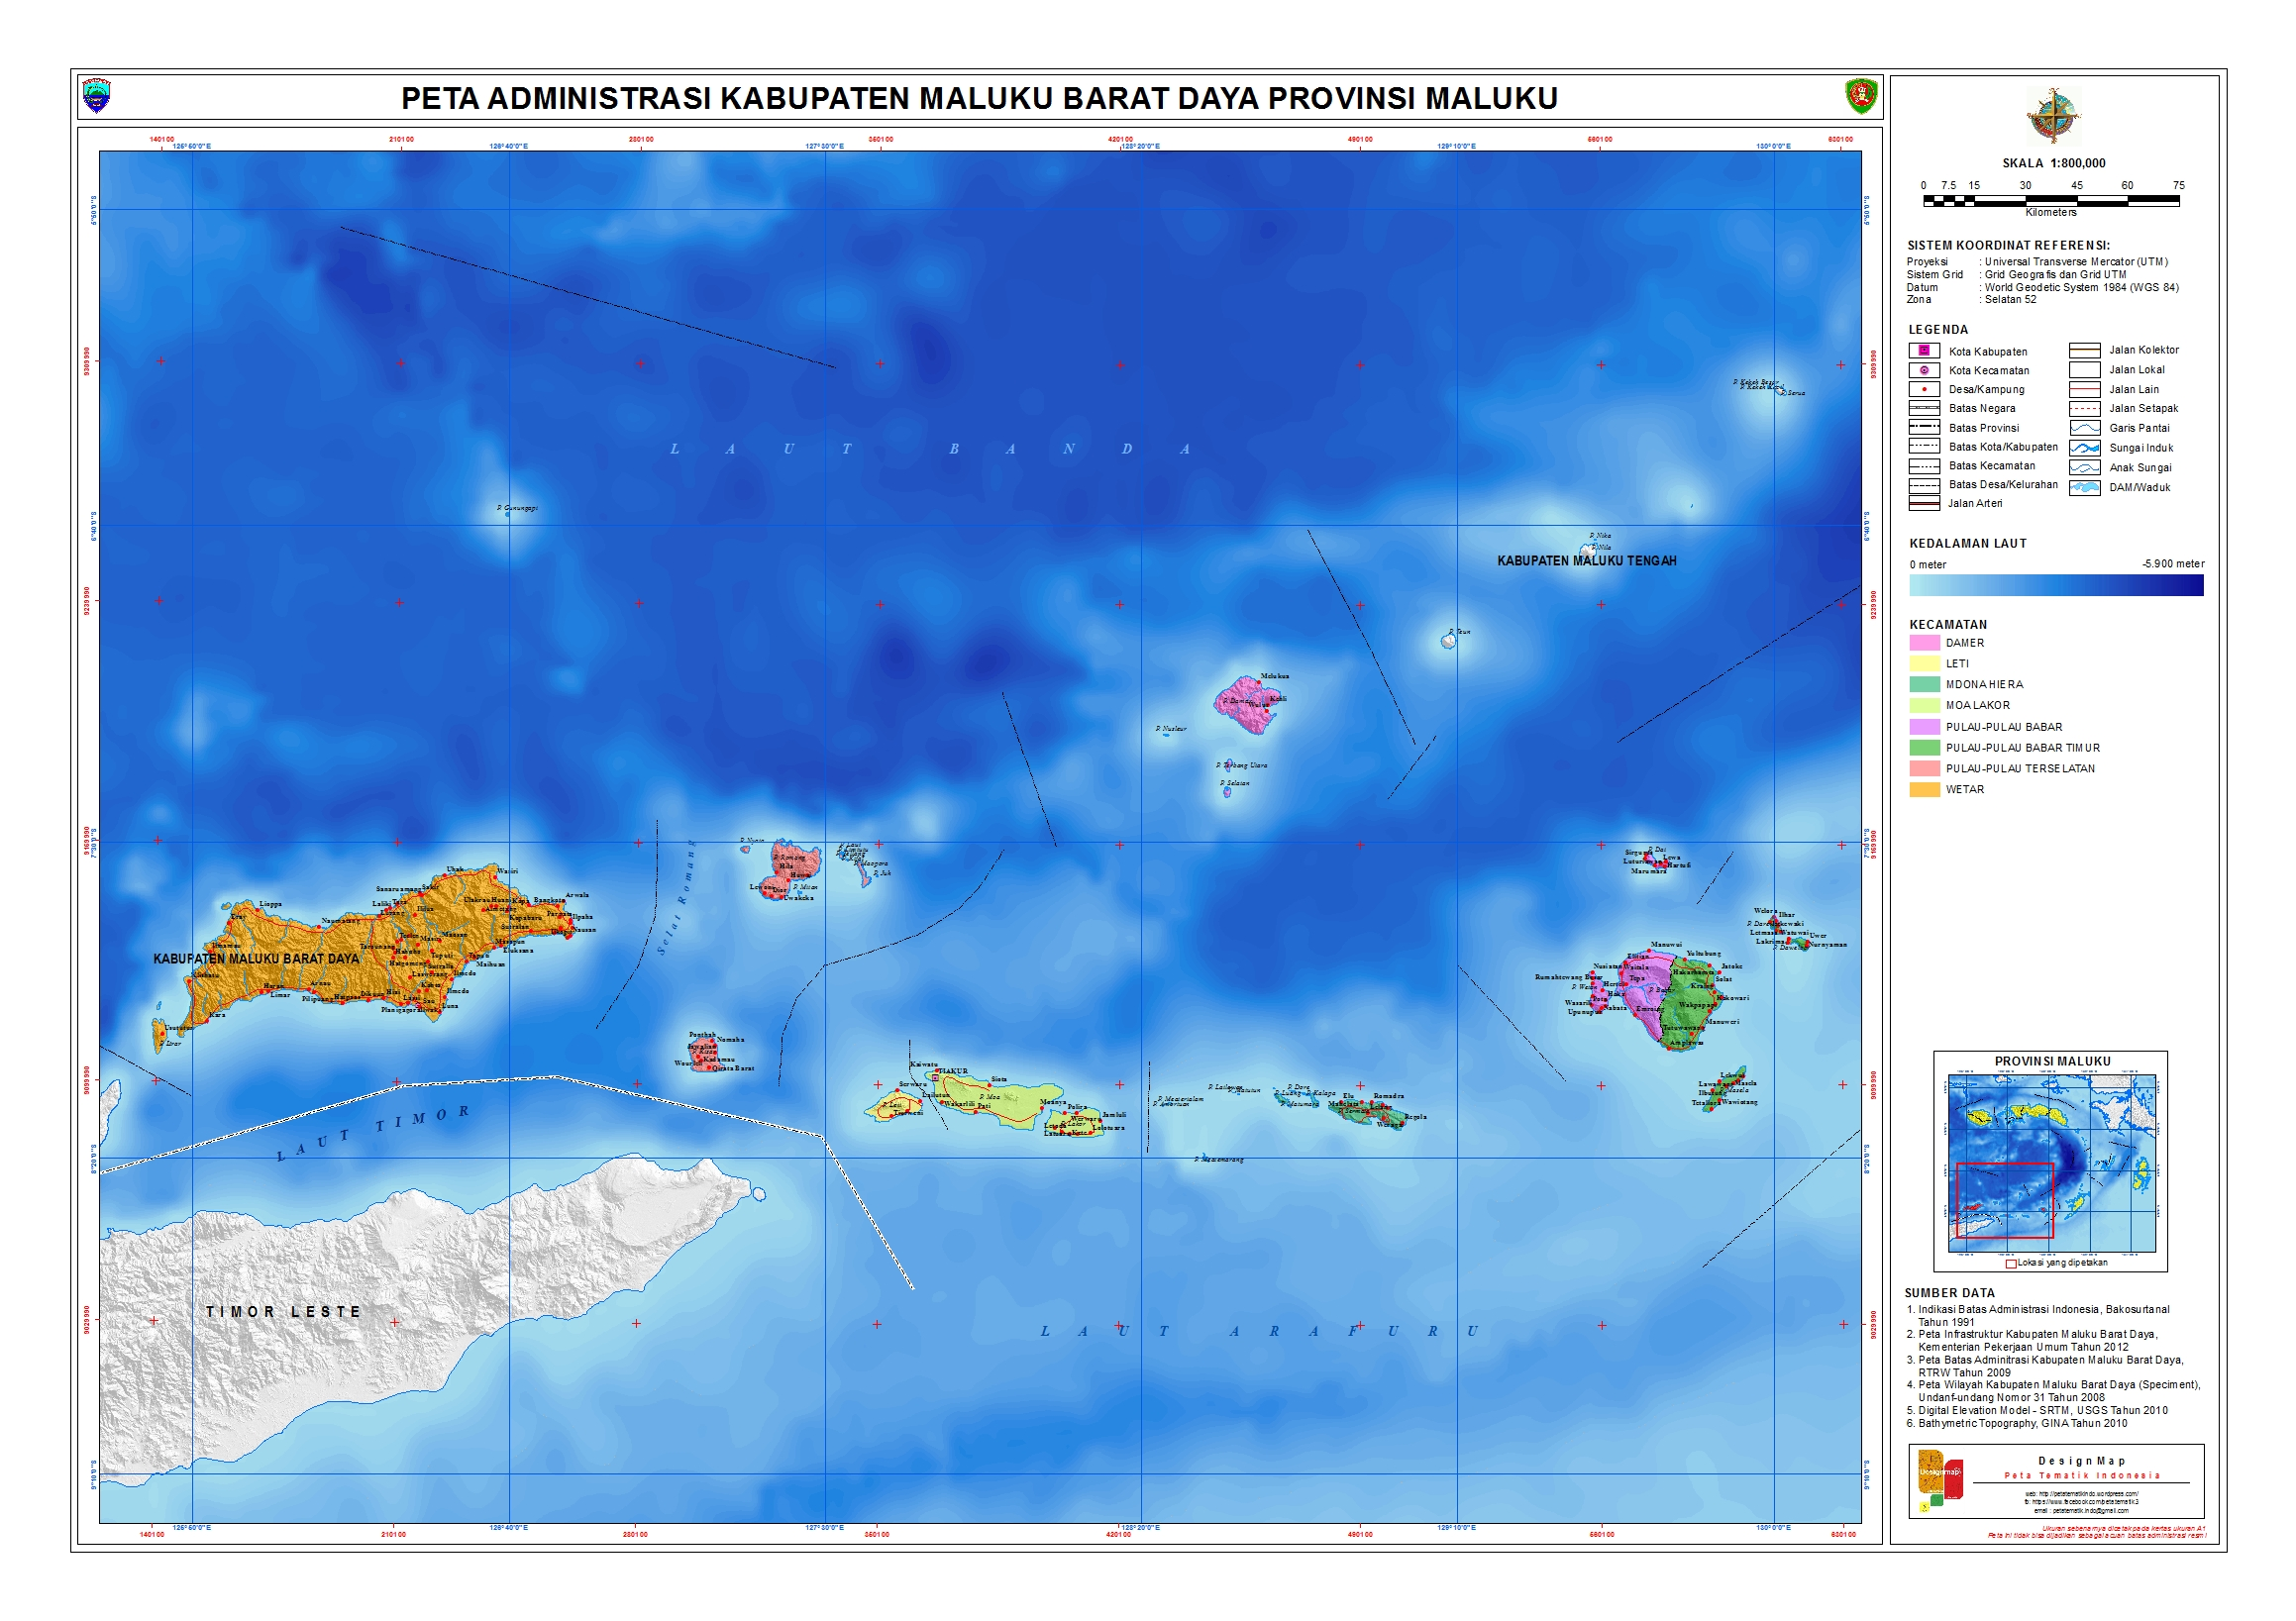
\includegraphics[width=0.8\textwidth]{gambar/administrasi-maluku-barat-daya-a1.jpg}
    \caption{Grafik Kuota dan Realisasi BBM Kabupaten Maluku Barat Daya Tahun 2021 \citep{Pertamina_2021}}
    \label{fig:realisasi-bbm-mbd}
\end{figure}

    Pemasokan BBM Kabupaten MBD saat ini dilayani oleh tiga kapal yaitu SPOB Handil Tirusan, SPOB Cinta Damai dan LCT Buma III.
    Sistem penyaluran bersifat \emph{direct} dari TBBM Saumlaki menuju 5 titik pemasokan yaitu Tiakur, Tepa, Lakor, Letti dan Romang. Ilustrasi rute dapat dilihat pada gambar \ref{fig:rute-old-bbm-mbd}. Warna merah muda melambangkan kapal SPOB Handil Tirusan, Hijau adalah SPOB Cinta Damai dan Biru adalah LCT BUMA III.

\begin{figure}[htbp!]
    \centering
    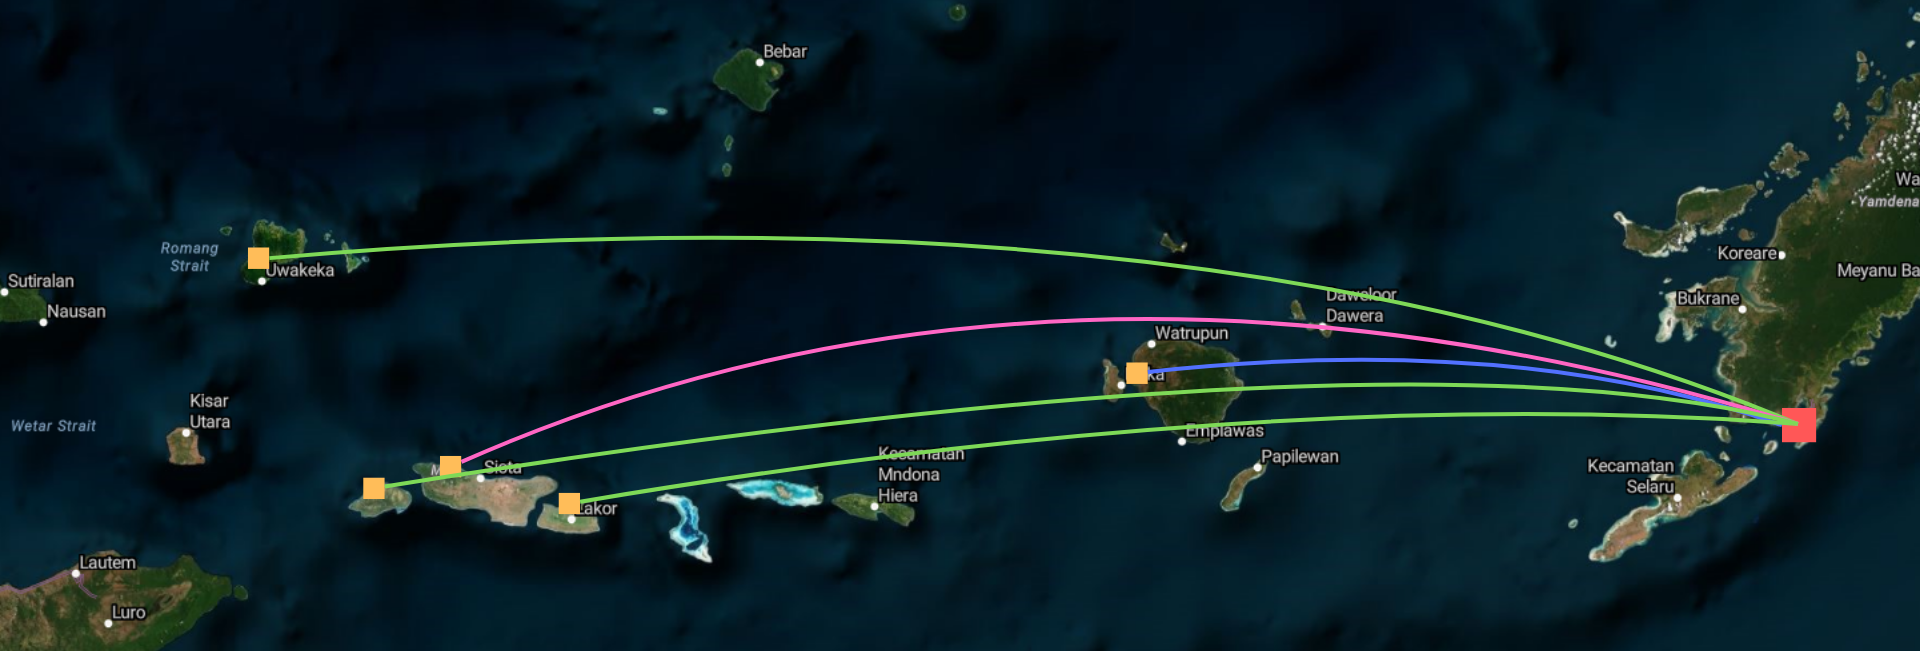
\includegraphics[width=0.8\textwidth]{gambar/rute-eksisting.png}
    \caption{Pola Operasi Pemasokan BBM Kabupaten MBD Saat Ini}
    \label{fig:rute-old-bbm-mbd}
\end{figure}

    SPOB Cinta Damai melayani tiga titik pasokan yaitu Letti, Romang dan Lakor dengan rata-rata muatan 75 kiloliter. SPOB Handil Tirusan melayani titik Tiakur dengan rata-rata muatan 50 kiloliter. LCT BUMA III melayani titik Tepa dengan rata-rata muatan 50 kiloliter. Ringkasan penyaluran BBM berdasarkan moda kapal dapat dilihat pada gambar 

\begin{figure}[htbp!]
    \centering
    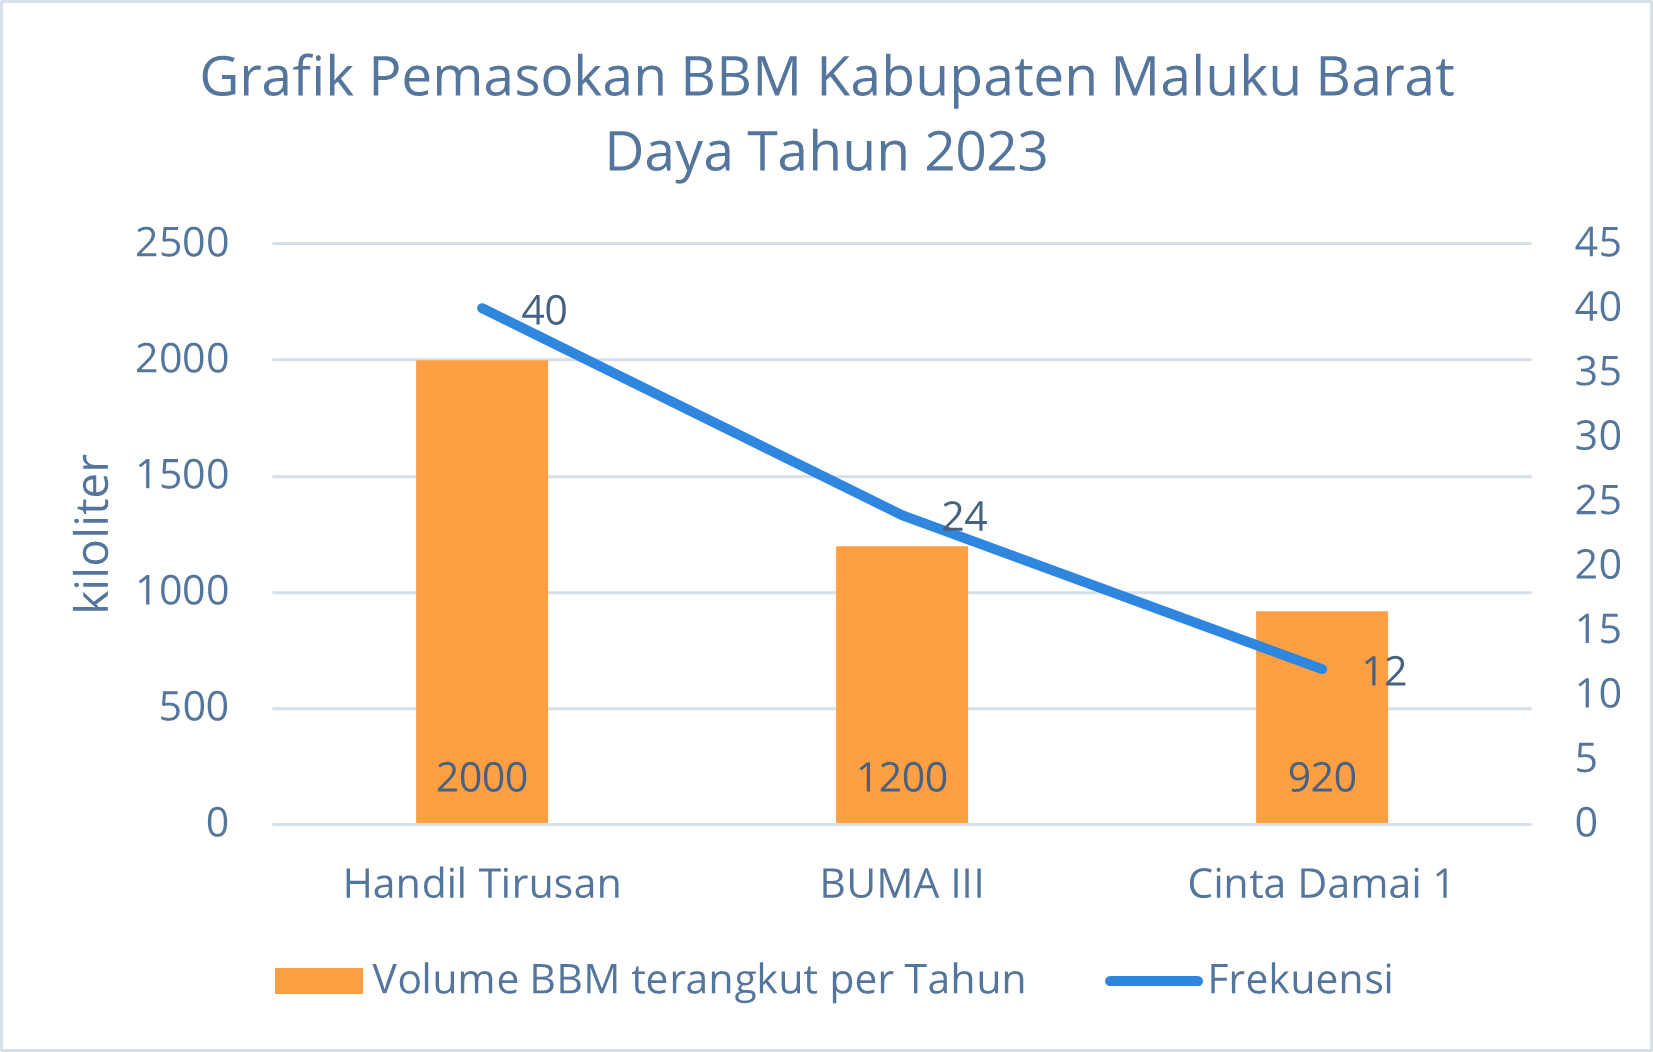
\includegraphics[width=0.8\textwidth]{gambar/pemasokan-BBM-MBD.png}
    \caption{Grafik Pemasokan BBM Kabupaten Maluku Barat Daya Tahun 2023 berdasarkan kapal}
    \label{fig:kapal-mbd-old}
\end{figure}